\section{Extensions of linear models}


\newcommand{\datasetplot}[1]{
    \begin{tikzpicture}
        \begin{axis}[
            height=5cm,
            width=8cm,
            xmin=0,
            xmax=1,
            xtick pos=bottom,
            ytick pos=left,
            ymajorticks=false
        ]
            \ifnum#1=0
                \addplot[
                    only marks,
                    blue,
                    samples=100,
                    domain=0:1,
                    opacity=0.5
                ] (x, 20 + 5 * x + rand);
            \fi
            \ifnum#1=1
                \addplot[
                    only marks,
                    blue,
                    samples=100,
                    domain=0:1,
                    opacity=0.5
                ] (x, 20 + x^3 * 5 + rand);
            \fi
            \ifnum#1=2
                \addplot[
                    only marks,
                    blue,
                    samples=100,
                    domain=-1:1,
                    opacity=0.5
                ] coordinates {
                    (0.1, 0)
                    (0.15, 0)
                    (0.22, 0)
                    (0.4, 0)
                    (0.25, 0)
                    (0.55,0)
                    (0.43, 0)
                    (0.51, 0)
                };
                \addplot[
                    only marks,
                    blue,
                    samples=100,
                    domain=-1:1,
                    opacity=0.5
                ] coordinates {
                    (0.3, 1)
                    (0.47, 1)
                    (0.52, 1)
                    (0.65, 1)
                    (0.81, 1)
                    (0.84,1)
                    (0.91, 1)
                    (0.99, 1)
                };
            \fi
            \ifnum#1=3
                \addplot[
                    only marks,
                    blue,
                    samples=100,
                    domain=-1:1,
                    opacity=0.5
                ] coordinates {
                    (0.1, 0)
                    (0.15, 0)
                    (0.22, 0)
                    (0.4, 0)
                    (0.25, 0)
                    (0.55,0)
                    (0.43, 0)
                    (0.51, 0)
                };
                \addplot[
                    only marks,
                    blue,
                    samples=100,
                    domain=-1:1,
                    opacity=0.5
                ] coordinates {
                    (0.3, 1)
                    (0.47, 1)
                    (0.52, 1)
                    (0.65, 1)
                    (0.81, 1)
                    (0.84,1)
                    (0.91, 1)
                    (0.99, 1)
                };
                \addplot[
                    domain=0:1,
                    samples=100,
                    thick,
                    red
                ] {1 / (1 + exp(-(20 * (x - 0.5))))};
            \fi
            \ifnum#1=4
                \addplot[
                    only marks,
                    blue,
                    samples=100,
                    domain=0:1,
                    opacity=0.5
                ] (x, 20 + x^3 * 5 + rand);
                \addplot[
                    thick,
                    red,
                    samples=100,
                    domain=0:1
                ] (x, 20+x^3*5);
            \fi
        \end{axis}
    \end{tikzpicture}
}

\newsavebox{\linearbox}
\sbox{\linearbox}{
    \datasetplot{0}
}

\newsavebox{\exponentialbox}
\sbox{\exponentialbox}{
    \datasetplot{1}
}

\newsavebox{\logisticbox}
\sbox{\logisticbox}{
    \datasetplot{2}
}

\newsavebox{\logregbox}
\sbox{\logregbox}{
    \datasetplot{3}
}

\newsavebox{\expregbox}
\sbox{\expregbox}{
    \datasetplot{4}
}

\begin{frame}{Extensions of linear models: Motivation}
    \begin{tikzpicture}
        \node[draw=black] at (-5.25, -3.5) {};
        \node[draw=black] at (5.25, 3.5) {};

        \visible<1-3,5>{
            \node[] at (0, -2.5) {
                $\hat{y}=$$\beta_0+\sum\limits_{i=0}^p \beta_ix_i$
            };
        }

        \visible<2>{
            \node[] at (0, 1) {
                \usebox{\linearbox}
            };
        }
        \visible<3-4,12>{
            \node[] at (0, 1) {
                \usebox{\exponentialbox}
            };
        }
        \visible<4>{
            \node[] at (0, -2.5) {
                $\hat{y}=$\textcolor{red}{$\beta_0+\sum\limits_{i=0}^p \beta_ix_i$}
            };
        }
        \visible<5-7>{
            \node[] at (0, 1) {
                \usebox{\logisticbox}
            };
        }
        \visible<6>{
            \node[] at (0, -2.5) {
                $\log\left(\dfrac{p(X)}{1 - p(X)}\right)=\beta_0+\sum\limits_{i=0}^p \beta_ix_i$
            };
        }
        \visible<7-8>{
            \node[] at (0, -2.5) {
                $p(X)=\dfrac{e^{\left(\beta_0+\sum\limits_{i=0}^p \beta_ix_i\right)}}{1 + e^{\left(\beta_0+\sum\limits_{i=0}^p \beta_ix_i\right)}}$
            };
        }
        \visible<8-11>{
            \node[] at (0, 1) {
                \usebox{\logregbox}
            };
        }
        \visible<9>{
            \node[] at (0, -2.5) {
                $p(X)=\dfrac{e^{\left({\color{red}\beta_0+\sum\limits_{i=0}^p \beta_ix_i} \right)}}{1 + e^{\left({\color{red}\beta_0+\sum\limits_{i=0}^p \beta_ix_i}\right)}}$
            };
        }
        \visible<10>{
            \node[] at (0, -2.5) {
                $p(X)=f(\beta_0+\sum\limits_{i=0}^p \beta_ix_i)$
            };
        }
        \visible<11-12>{
            \node[] at (0, -2.5) {
                $f(\hat{y})=\beta_0+\sum\limits_{i=0}^p \beta_ix_i$
            };
        }
        \visible<13>{
            \node[] at (0, 1) {
                \usebox{\expregbox}
            };
            \node[] at (0, -2.5) {
                $\log(\hat{y})=\beta_0+\sum\limits_{i=0}^p \beta_ix_i$
            };
        }
        \visible<14>{
            \node[align=flush left, text width=10.5cm] at (0, 0) {
                \textbf{Generalized linear models (GLMs):}\\
                Extends upon the regular linear model by associating the predictors to the response via a non-linear link function.
            };
        }
    \end{tikzpicture}
\end{frame}
